\documentclass[11pt]{article}
\usepackage{fullpage}
\usepackage{amsthm}
\usepackage{amsmath}
\usepackage{amssymb}
\usepackage{graphicx}

\graphicspath{ {./imgs/} }

\setlength{\parindent}{0pt}

\title{Robotics (CO333)}
\author{Michael Tsang}

\newtheorem{defn}{Definition}
\newtheorem{eg}{Example}
\newtheorem{theo}{Theorem}
\newtheorem{lem}{Lemma}

\begin{document}

\maketitle

\section{Robot Motion}
A mobile robot can move and sense, and must process information to link these two.

What are the possible goals of a robot locomotion system?
\begin{itemize}
  \item Speed and/or acceleration of movement.
  \item Precision of positioning (repeatability).
  \item Flexibility and robustness in different conditions.
  \item Efficiency.
\end{itemize}

Robots could move in water, air, land, or even space.
We focus on wheeled robots which move on fairly flat surfaces.

\subsection{Motion and Coordinate Frames}
We define two coordinate frames: a \textbf{world frame} $W$ anchored in the world and a \textbf{robot frame} $R$ which is carried by and stays fixed relative to the robot at all times.

We are interested in the robot's \textbf{location}: the transformation between $W$ and $R$.

\subsection{Degrees of Motion Freedom}
A rigid body which translates and rotates along a:
\begin{itemize}
  \item 1D path has 1 degree of freedom (DOF): 1 translational.
  \item 2D plane has 3 DOF: 2 translational, 1 rotational.
  \item 3D volume has 6 DOF: 3 translational, 3 rotational.
\end{itemize}

A \textbf{holonomic robot} is one which is able to move instantaneously in any direction in the space of its degrees of freedom.

Although holonomic robots exist, they need many motors or unusual designs, and are often impractical.

\subsection{Wheel Configurations}
\begin{itemize}
  \item Rack and Pinion.
  \item Differential Drive.
  \item Skid-Steer.
  \item Synchro Drive.
\end{itemize}
These are standard non-holonomic configurations and are simple, reliable, robust mechanisms suitable for robots which essentially move in a plane.

Some more exotic non-holonomic configurations are:
\begin{itemize}
  \item Segway - good height with small footprint and high acceleration; self balancing.
  \item Mars Rover - wheels on stalks to tackle large obstacles.
\end{itemize}

\subsection{Differential Drive}
\begin{itemize}
  \item Two motors, one per wheel.
  \item Steer by setting different speeds on each wheel.
  \item Wheels run at equal speeds for straight-line motion.
  \item Wheels run at equal and opposite speeds to turn on the spot.
  \item Other combinations of speeds allow circular arcs.
\end{itemize}

\subsection{Circular Path of a Differential Drive Robot}
\begin{figure}[h]
  \caption{Differential Drive Robot}
  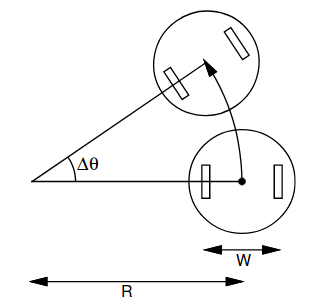
\includegraphics[scale=0.4]{ddrobot}
  \centering
\end{figure}

Let the wheel velocities of the left and right wheels respectively be $v_L$ and $v_R$.
These are linear velocities of the wheels over the ground: $v_X = r_X\omega_X$, where $r_X$ is the radius of the $X$ wheel and $\omega_X$ is its angular velocity.

The width between the wheels is $W$.

\begin{itemize}
  \item Straight line motion if $v_L = v_R$.
  \item Turns on the spot if $v_L = - v_R$.
\end{itemize}

To find radius $R$ of a curved path, consider a period of motion $\Delta t$ where the robot moves along a circular arc through angle $\Delta \theta$.
\begin{itemize}
  \item Left wheel: $\text{distance moved } = v_L \Delta t$; $\text{radius of arc } = R - \frac{W}{2}$.
  \item Right wheel: $\text{distance moved } = v_R \Delta t$; $\text{radius of arc } = R + \frac{W}{2}$.
  \item Both wheel arcs subtend the same angle so:
    \[
      \Delta \theta = \frac{v_L \Delta t}{R - \frac{W}{2}} = \frac{v_R \Delta t}{R + \frac{W}{2}}
    \]
    \[
      \implies \frac{W}{2}(v_L + v_R) = R(v_R - v_L)
    \]
    \begin{align*}
      \implies R &= \frac{W(v_R + v_L)}{2(v_R - v_L)} & \Delta \theta &= \frac{(v_R - v_L)\Delta t}{W}
    \end{align*}
\end{itemize}

\subsection{Rack and Pinion Drive (Car/Tricycle)}
\begin{figure}[h]
  \caption{Rack and Pinion Drive layouts.}
  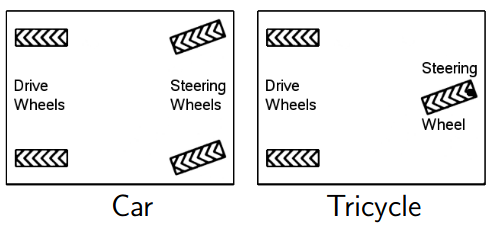
\includegraphics[scale=0.4]{piniondrive}
  \centering
\end{figure}

\begin{itemize}
  \item Two motors: one to drive, one to steer.
  \item Cannot normally turn on the spot.
  \item With fixed speed and steering angle, will follow a circular path.
  \item With four wheels, need rear differential and variable (``Ackerman'') linkage for steering wheels.
\end{itemize}

\subsection{Circular Path of a Car-Like Tricycle Robot}
\begin{figure}[h]
  \caption{Tricycle Robot.}
  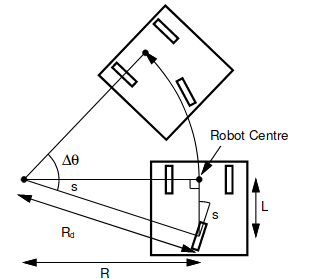
\includegraphics[scale=0.5]{tricycle}
  \centering
\end{figure}

Single steerable and drivable wheel at back, front wheels are free running.

Assuming no sideways wheel slip, we intersect the axes of the front and back wheels to forma right-angle triangle:
\[
  R = \frac{L}{\tan s}
\]

The radius of the path the rear wheels moves is:
\[
  R_d = \frac{L}{\sin s}
\]

In time $\Delta t$, the distance along its circular arc moved by the wheel is $v\Delta t$, so the angle $\Delta \theta$ through which the robot rotates is:
\[
  \Delta \theta = \frac{v\Delta t}{R_d} = \frac{v\Delta t \sin s}{L}
\]

\subsection{Gearing}
\begin{figure}[h]
  \caption{Gears of a DC motor.}
  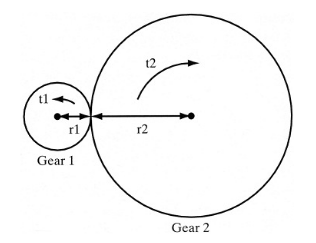
\includegraphics[scale=0.5]{gearing}
  \centering
\end{figure}

DC motors offer high speed and low torque, so gearing is nearly always required to drive a robot.

If Gear 1 is driven with torque $t_1$, it exerts tangential force:
\[
  F = \frac{t_1}{r_1}
\]

on Gear 2; the torque in Gear 2 is therefore:
\[
  t_2 = r_2F = \frac{r_2}{r_1}t_1
\]

The change in angular velocity between Gear 1 and Gear 2 is calcualted by considering velocity at the point where they meet:
\[
  v = \omega_1 r_1 = \omega_2 r_2
\]
\[
  \implies \omega_2 = \frac{r_1}{r_2}\omega_1
\]
\begin{itemize}
  \item When a small gear drives a bigger gear, the second gear has higher torque and lower angular velocity in proportion to the ratio of teeth.
  \item Gears can be chained together to achieve compound effects.
\end{itemize}

\subsection{Motor Control - Open Loop}
\begin{figure}[h]
  \caption{Open loop system.}
  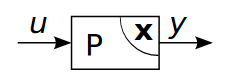
\includegraphics[scale=0.4]{openloop}
  \centering
\end{figure}

Let $P$ be a Single-Input-Single-Output (SISO) dynamic system, it is described by:
\begin{itemize}
  \item An input $u$ - here: voltage $V$, or corresponding Pulse Width Modulation (PWM) value.
  \item Internal states $x$, whose dynamics follow differential equations - here: $x = [x_1, x_2]^\top = [\omega, \varphi]^\top$, with rotation speed $\omega$ and angle $\varphi$.
  \item An output $y$ as a function of $x$ - here: angle $\varphi$, $y = x_2$.
\end{itemize}

Qualitative open-loop response on input (voltage) step: input $V$ leads to output motor angle $\phi$, which changes with time.

\subsection{Motor Control - Closed Loop}
\begin{figure}[h]
  \caption{Closed loop system.}
  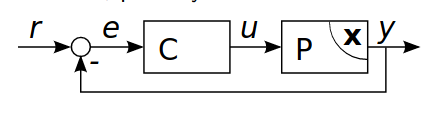
\includegraphics[scale=0.4]{closedloop}
  \centering
\end{figure}

Let $C$ be a controller possibly with internal states:
\begin{itemize}
  \item $r$ is a reference (desired) output.
  \item $e$ is the e  rror between reference and actual output.
\end{itemize}

The controller runs at a high frequency, at each iteration it checks the current error and calculates a control value to the motor which aims to reduce the error.

This is simple: a binary on or off.

\subsection{General Motor Control - PID}
Proportional-Integral-Differential (PID), a controller:
\[
  C : u(t) = k_p \exp(t) + k_i \int_{t_0}^{t} \exp(\tau)d_\tau + k_d \frac{d\exp(t)}{dt}
\]
where
\begin{itemize}
  \item $k_p$ - proportional gain, reduces the error.
  \item $k_i$ - integral gain, removes steady-state error.
  \item $k_d$ - differential gain, can reduce settling time.
\end{itemize}

A simple (heuristic) tuning rule is the \textbf{Ziegler-Nichols}:
\begin{itemize}
  \item Set $k_i$ and $k_d$ to zero.
  \item Increase $k_p$ until the system starts oscillating with Period $P_u$ (in seconds) - remember this gain as $k_u$.
  \item Set $k_p = 0.6k_u, k_i = 2k_p/P_u, \text{and } k_d = k_pP_u/8$.
\end{itemize}

\subsection{Motor Control - Additional Tweaks}
\begin{itemize}
  \item Reference filtering - respect physical limits already in reference.
  \item Anti-Reset-Windup - stops integrating the effor for the I-part, when $u$ is at its physical limit.
  \item Dead-band compensation - add offset to $u$ to compensate friction.
  \item Feed-forward controller - $C_f : u_f(t) = k_f \frac{dr(t)}{dt}$, reduces ``work'' for the feedback controller
\end{itemize}

\subsection{Mapping Wheel Rotation Speed to Velocity}
In principle, we could emasure the radius of each wheel $r_W$ to turn angular into linear motion.
However in practice, due to hard to model factors, it is better to calibrate empirically, i.e.\ work out the scaling between the motor reference angle and the distance travelled over the ground via experiments.

\subsection{Motion and State on a 2D Plane}
We can define a \textbf{state vector} $\textbf{x}$:
\[
  \textbf{x} = 
  \begin{pmatrix}
    x \\ y \\ \theta
  \end{pmatrix}
\]
\begin{itemize}
  \item $x$ and $y$ specify the location of the pre-define ``robot centre'' point in the world frame.
  \item $\theta$ specifies the rotation angle between the two coordinate frames (the angle between the $x^W$ and $x^R$ axes).
  \item At the origin, $x = y = \theta = 0$.
\end{itemize}

\subsection{Integrating Motion in 2D}
2D motion on a plane: three degrees of position freedom $(x, y, \theta)$, with $-\pi < \theta \leq \pi$.

Consider a robot which either drives ahead or turns on the spot:
\begin{itemize}
  \item During straight-line period of motion of distance $D$:
    \[
      \begin{pmatrix}
        x_{\text{new}} \\
        y_{\text{new}} \\
        \theta_{\text{new}} 
      \end{pmatrix}
      =
      \begin{pmatrix}
        x + D\cos\theta \\
        y + D\sin\theta \\
        \theta 
      \end{pmatrix}
    \]
  \item During a pure rotation of angle $\alpha$:
    \[
      \begin{pmatrix}
        x_{\text{new}} \\
        y_{\text{new}} \\
        \theta_{\text{new}} 
      \end{pmatrix}
      =
      \begin{pmatrix}
        x \\
        y \\
        \theta + \alpha
      \end{pmatrix}
    \]
\end{itemize}

\subsection{Integrating Circular Motion Estimates in 2D}
\begin{figure}[h]
  \caption{Circular Motion estimation.}
  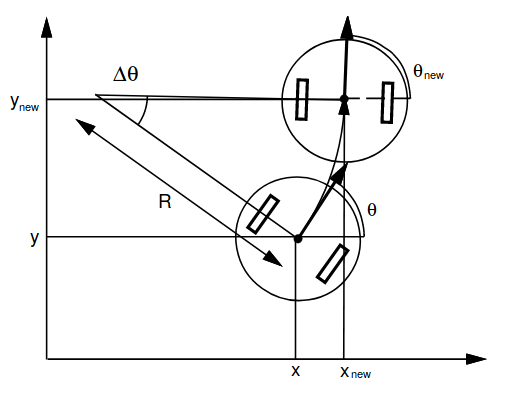
\includegraphics[scale=0.4]{circularmotionestimate}
  \centering
\end{figure}

\[
  \begin{pmatrix}
    x_{\text{new}} \\
    y_{\text{new}} \\
    \theta_{\text{new}} 
  \end{pmatrix}
  =
  \begin{pmatrix}
    x + R(\sin(\Delta \theta + \theta) - \sin \theta) \\
    y - R(\cos(\Delta \theta + \theta) - \cos \theta) \\
    \theta + \Delta \theta
  \end{pmatrix}
\]

\subsection{Position-Based Path Planning}
Assuming that robot has localisation and knows where it is relative to a fixed coordinate frame, then \textbf{position-based path planning} allows it to move in precise way along a sequence of pre-defined waypoints.
Paths of various curved shapes could be planning, aiming to optimise criteria (e.g.\ time or power).

We assume that:
\begin{itemize}
  \item Movements are composed by straight-line segments separated by turns on the spot.
  \item Total distance travelled is minimised - it always faces to turn the next waypoint and drive straight towards it.
\end{itemize}

If the current pose is $(x, y, \theta)$ and the next waypoint is $(W_x, W_y)$, it must first rotate to point towards the waypoint at vector direction:
\[
  \begin{pmatrix}
    d_x \\
    d_y
  \end{pmatrix}
  =
  \begin{pmatrix}
    W_x - x \\
    W_y - y
  \end{pmatrix}
\]
The absolute angular orientation $\alpha$ the robot must drive in is:
\[
  \alpha = \tan^{-1} \frac{d_x}{d_y}
\]

Care must be taken to ensure $\alpha$ is in the correct quadrant of $-\pi < \alpha \leq \pi$.

The angle the robot must rotate through is therefore $\beta = \alpha - \theta$.
To move as efficiently as possible, care should be taken to shift this angle by adding or subtracting $2\pi$ to ensure $-\pi < \beta \leq \pi$.

The robot should then drive forward straight for
\[
  d = \sqrt{d_x^2 + d_y^2}
\]

\section{Sensors}
\subsection{A Well Calibrated Robot}
After careful calibration, a robot should move to the desired location on average, but scatter will remain due to uncontrollable factors (e.g.\ wheel slip, rough surfaces).
Although \textbf{systematic error} may have been removed, \textbf{zero mean errors} still remain.

The errors occur incrementally: small additional movements/rotations induce slightly more potential error.

We can model the zero mean errors probabilistically, usually a Gaussian (normal) distribution.

\subsection{Uncertainty in Motion}
We modify the previous equations to acknowledge the uncertain perturbations:
\[
  \begin{pmatrix}
    x_{\text{new}} \\
    y_{\text{new}} \\
    \theta_{\text{new}} 
  \end{pmatrix}
  =
  \begin{pmatrix}
    x + (D + e)\cos\theta \\
    y + (D + e)\sin\theta \\
    \theta + f
  \end{pmatrix}
\]
\[
  \begin{pmatrix}
    x_{\text{new}} \\
    y_{\text{new}} \\
    \theta_{\text{new}} 
  \end{pmatrix}
  =
  \begin{pmatrix}
    x \\
    y \\
    \theta + \alpha + g
  \end{pmatrix}
\]

Here, $e, f, g$ are uncertainty terms with zero mean and Gaussian distribution, they model how the actual motion may deviate from the ideal trajectory.

These equations will be helpful when we probabilistically combine odometry with other sensing.

\subsection{Sensor Types}
Sensors are either \textbf{proprioceptive} (self-sensing) or \textbf{exteroceptive} (outward-looking).
\begin{itemize}
  \item Proprioceptive sensors (e.g.\ motor encoders, internal force sensors) improve a robot's sense of its own internal state and motion.
  \item Without exteroceptive sensors, a mobile robot moves blindly, it needs to:
    \begin{itemize}
      \item Localise without drift and with respect to a map.
      \item Recognise places and objects it has seen before.
      \item Map out free space, avoid obstacles.
      \item Interact with objects and people.
      \item Be aware of its environment.
    \end{itemize}
\end{itemize}

\subsection{Sensor Measurements: Proprioceptive}
\begin{itemize}
  \item Sensors gather numerical readings or \textbf{measurements}; for proprioceptive sensors, the value of the measurement $z_p$ will depend on just the state of the robot $x$:
    \[
      z_p = z_p(x)
    \]
  \item The state of a robot is a vector of variables describing its current status.
  \item More generally, a proprioceptive measurement might depend not just on the current state but also on previous states or the current rate of change of state.
\end{itemize}

\subsection{Sensor Measurements: Exteroceptive}
\begin{itemize}
  \item A measurement from an exteroceptive sensor depends on both the state of the robot $x$ and the world $y$:
    \[
      z_o = z_o(x, y)
    \]
  \item The state of the world might be parameterised in many ways, e.g.\ a list of geometric coordinates of walls or landmarks, either uncertain or perfectly known.
\end{itemize}

\subsection{Single and Multiple Value Sensors}
\begin{itemize}
  \item Touch, light and sonar sensors return a singe value within a given range.
  \item Sensors such as a camera or laser range-finder return an array of values, achieved either by scanning a single sensing element or by having an array of sensing elements.
\end{itemize}

\subsection{Touch Sensor}
\begin{itemize}
  \item Binary on/off state - no processing required.
  \item Switch open - no current flow.
  \item Switch closed - current flow.
\end{itemize}

\subsection{Light Sensor}
\begin{itemize}
  \item Detect intensity of light incident from a single forward direction, with some range of angular sensitivity.
  \item Multiple sensors pointing in different directions can guide steering behaviours.
  \item The Lego sensors can also emit their own light, which reflect off close targets.
\end{itemize}

\subsection{Sonar (Ultrasonic) Sensor}
\begin{itemize}
  \item Measures depth by emitting an ultrasonic pulse and timing interval for echo to return.
  \item Fairly accurate in one direction but can give noisy measurements in the presence of complicated shapes.
  \item Ring of sonar sensors can be used for obstacle detection.
  \item Important for underwater robots as it is the only serious option beyond very short ranges.
\end{itemize}

\subsection{External Sensing: Laser Range-Finder}
\begin{itemize}
  \item Measures depth using an active signal; commercial LADAR sensors return an array of depth measurements from a scanning beam.
  \item Very accurate measurement depth, works on most surface types.
  \item Normally scans in a 2D plane.
  \item Bulky and expensive.
\end{itemize}

\subsection{External Sensing: Vision}
\begin{itemize}
  \item Generalisation of a light sensor - measures light intensity in many directions simultaneously by directing incident light onto a sensing chip with an array of sensitive elements.
  \item Returns large, rectangular array of measurements.
  \item A single camera measures light intensity, multiple cameras or a single moving one allows 3D information processing.
  \item Low cost.
\end{itemize}

\subsection{Touch Sensors for Bump Detection}
The sensor detects when an obstacle has been hit, demanding an immediate reaction (e.g.\ evasive manoeuvre or stopping motion).

For a circular robot, we can mount touch sensors inside a ``floating skirt'' to give the ability to measure different bump directions.

\begin{itemize}
  \item Stationary object collision: explore by reversing and trying to go around.
  \item Moving object collision: follow or run away.
\end{itemize}

\subsection{Servoing}
\textbf{Servoing} is a robot control technique where control parameters are coupled directly to a sensor reading and updated regularly in a \textbf{negative feedback loop}, sometimes known as \textbf{closed loop control}.

Servoing requires high frequency update of sensor/control cycle, otherwise motion may oscillate.

\subsection{Exteroceptive Servoing}
In servoing, a control demand is set which over time aims to bring the current value of a sensor reading to agree with a desired value.

\textbf{Proportional control:} set demand proportional to negative error (difference between desired value and actual value).
\[
  -k_p(z_{\text{desired}} - z_{\text{actual}})
\]
where $k_p$ is the proportional gain constant.

\begin{itemize}
  \item \textbf{Cascade control} is where the output of one control loop is used to set the input to another, hiding the details of motor/encoder control from the upper level work with sensor control. 
  \item Problems only arise when the top level controller requests changes too rapidly, exceeding the \textbf{bandwidth} of lower level controllers.
  \item Sensors may sometimes produce garbage readings for a number of different possible reasons; it is often sensible to use a strategy to remove outliers but this also reduces the responsiveness of the system.
\end{itemize}

\subsection{Visual Servoing to Control Steering}

\begin{figure}[h]
  \caption{Steering for a robot with a tricycle or car-type wheel configuration.}
  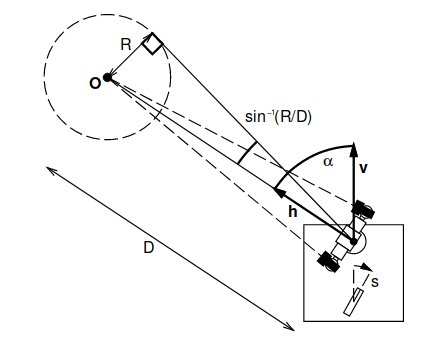
\includegraphics[scale=0.4]{steering}
  \centering
\end{figure}

Simple steering law to collide with target:
\[
  s = k_p \alpha
\]
  
Steering law to avoid obstacle at safe radius:
\[
  s = k_p (\alpha - \sin^{-1} \frac{R}{D})
\]

\subsection{Combining: Sensing/Action Loops}
We consider each local ``servo''-like sensing-action loop as a \textbf{behaviour}, we do not model or plan.

Sense $\rightarrow$ Act.

The challenge is combining many behaviours into useful overall activity.

\subsection{Combining: World Model Approach}
\begin{itemize}
  \item Capture data, store, and manipulate using symbolic representations.
  \item Plan a sequence of actions to achieve a given goal.
  \item Execute plan.
  \item If world changes during execution, stop and re-plan.
\end{itemize}

This is powerful, but computationally expensive and complicated.

Probabilistic state inference and planning is the modern version of this, and able to cope with uncertainty in sensors.

\subsection{Probabilistic Sensor Modelling}
Robot sensing, like motion, is fundamentally uncertain.
Real sensors do not report the exact truth but a perturbed version.

Having characterised (modelled, calibrated) a sensor and understood the uncertainty in measurements, we can build a probabilistic measurement model for how it works.
This is a \textbf{likelihood function}:
\[
  p(z_o \mid x, y)
\]
which often has a Gaussian shape.

\subsection{Likelihood Functions}
A \textbf{likelihood function} fully describes a sensor's performance.

$p(z \mid v)$ is a function of both measurement variables $z$ and ground truth $v$, and can plotted as a probability surface.

\begin{figure}[h]
  \caption{Probability surfaces for a depth sensor.}
  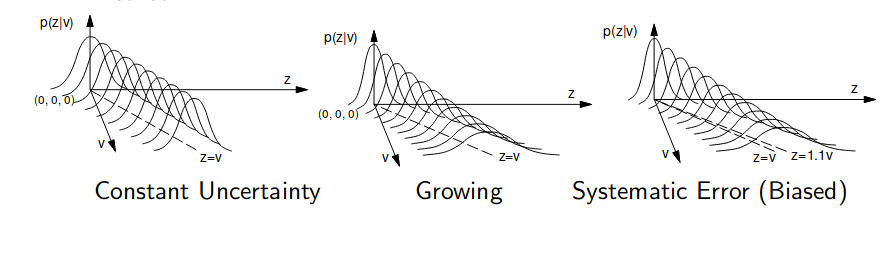
\includegraphics[scale=0.4]{uncertainty}
  \centering
\end{figure}

\section{Probabilistic Robots}
Problem: simple sensing/action procedures can be locally effective but are limited; we need longer-term representations and consistent scene models.

Classical AI approaches (logical reasoning) fail with real-world data:
\begin{itemize}
  \item Advanced sensors do not lend themselves to straightforward analysis.
  \item All information received is uncertain.
\end{itemize}

A probabilistic approach acknowledges uncertainty and uses models to abstract useful information from data - our goal is an incrementally updated probabilistic estimate of the position of the robot relative to the map.

\subsection{Uncertainty in Robotics}
\begin{itemize}
  \item Every robot action is uncertain.
  \item Every sensor measurement is uncertain.
  \item When we combine actions adn measurements to estimate state, the state estimate will be uncertain.
\end{itemize}

Usually, we start with an uncertain state estimate, take some action, receive new sensor information, then must update the uncertain state estimate in response.

\subsection{Probabilistic Inference}
What is my state and that of the world around me?
\begin{itemize}
  \item Prior knowledge is combined with new measurements, generally modelled as a \textbf{Bayesian Network}.
  \item Series of weighted combinations of old and new measurements.
  \item \textbf{Sensor fusion} - combining data from many different sources into useful estimates.
  \item The composite state estimate can then be used to decide the next action.
\end{itemize}

\subsection{Bayesian Probabilistic Inference}
\begin{itemize}
  \item ``Bayesian'' - measure of subjective belief.
  \item Probabilities describe our state of knowledge, not randomness.
  \item \textbf{Bayes' Rule:}
    \[
      P(X \mid Z) = \frac{P(Z \mid X)P(X)}{P(Z)}
    \]
  \item $P(X)$ - \textbf{prior}; $P(Z \mid X)$ - \textbf{likelihood}; $P(X \mid Z)$ - \textbf{posterior}; ($P(Z)$ - \textbf{marginal likelihood}).
  \item We use Bayes' Rule to incrementally digest new information from sensors about a robot's state.
\end{itemize}

\subsection{Probability Distributions}
\begin{itemize}
  \item As we decrease bin size, discrete probabilistic inference generalises to large numbers of possible states, limiting to a continuous probability density function.
  \item Explicit Gaussian distributions often represent uncertainty in sensor measurements well.
  \item The Gaussian prior multiplied by the Gaussian likelihood produce a Gaussian posterior which is tighter than either.
  \item Particles are a finite set of weighted samples of the state.
  \item With a high number of particles, they can represent the shape of distribution in ambigiuous situations.
\end{itemize}

\subsection{Probabilistic Localisation}
\begin{itemize}
  \item The robot has a map of its environment in advance.
  \item The only uncertainty is the robot's position.
  \item The robot stores and updates a probability distribution representing its uncertain position estimate.
\end{itemize}

\subsection{Monte Carlo Localisation (Particle Filter)}
A cloud of particles represent uncertain robot states; the more particles in a region, the higher the probability the robot is there.

A particle is a point estimate $x_i$ of the state of the robot with weight $w_i$:
\[
  x_i = 
  \begin{pmatrix}
    x_i \\
    y_i \\
    \theta_i
  \end{pmatrix}
\]

The full particle set is:
\[
  \{ x_i, w_i \} \text{ for } i = 1..N \text{ (usually N = 100)}
\]

All weights should add up to 1, if so the distribution is \textbf{normalised}:
\[
  \sum_{i = 1}^N w_i = 1
\]

\subsection{Displaying a Particle Set}
\begin{figure}[h]
  \caption{Particle set representation}
  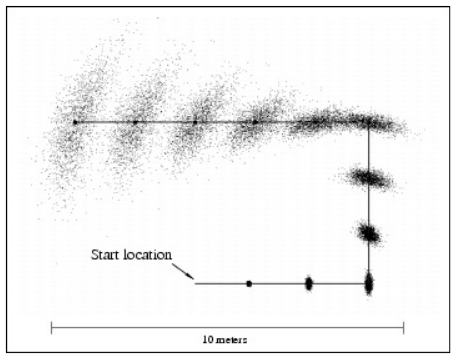
\includegraphics[scale=0.4]{particleset}
  \centering
\end{figure}

We visualise by plotting the $x$ and $y$ coordinates as a set of dots.
It is more difficult to visualise the $\theta$, but we can get the main idea from just the linear components.

\subsection{Steps in Particle Filtering}
\begin{enumerate}
  \item Motion Prediction based on Proprioceptive Sensors.
  \item Measurement Update based on Extereoceptive Sensors.
  \item Normalisation.
  \item Resampling.
\end{enumerate}

\subsection{Motion Prediction}
Uncertainty grows during blind motion.
When the robot makes a movement, the particle distribution shifts its mean position but also spreads out.

This is achieved by passing the state part of each particle through a function which has a deterministic and a random component.

During a straight-line period of motion of distance $D$:
\[
  \begin{pmatrix}
    x_{new} \\
    y_{new} \\
    \theta_{new}
  \end{pmatrix}
  =
  \begin{pmatrix}
    x + (D + e)\cos \theta \\
    y + (D + e)\sin \theta \\
    \theta + f
  \end{pmatrix}
\]

During a pure rotation of angle $\alpha$:
\[
  \begin{pmatrix}
    x_{new} \\
    y_{new} \\
    \theta_{new}
  \end{pmatrix}
  =
  \begin{pmatrix}
    x \\
    y \\
    \theta + \alpha + g
  \end{pmatrix}
\]

Here, $e, f, g$ are zero mean \textbf{noise} terms, random numbers with a Gaussian distribution which are generated for each particle, causing spread.

To set $e, f, g$, make initial estimates then adjust be looking at the particle spread over an extended motion and matching the distribution to experiments.

\subsection{Measurement Updates}
A measurement update consists of applying Bayes' Rule to each particle:
\[
  P(X \mid Z) = \frac{P(Z \mid X) P(X)}{P(Z)}
\]

When we achieve a measurement $z$, we update the weight of each particle as follows:
\[
  w_{i(new)} = P(z \mid x_i) \times w_i
\]
The denominator in Bayes' rule is a constant factor which will later be removed by normalisation so it is not calculated.

$P(z \mid x_i)$ is the likelihood of particle $i$, the probability of getting measurement $z$ given that it represents the true state.

\subsection{Likelihood Function}
The form of a likelihood function comes from a probabilistic model of the exteroceptive sensor.

Having calibrated a sensor and understood the uncertainty in its measurements, we can build a probabilistic measurement model for how it works:
\[
  P(z \mid x_i)
\]
This is a probability distribution (a likelihood function), often with a Gaussian shape.

\end{document}

